\documentclass[a4paper,12pt]{article}
\usepackage{amsmath}
\usepackage{amssymb}
\usepackage[polish]{babel}
\usepackage{polski}
\usepackage[utf8]{inputenc}
\usepackage{indentfirst}
\usepackage{geometry}
\usepackage{array}
\usepackage[pdftex]{color,graphicx}
\usepackage{subfigure}
\usepackage{afterpage}
\usepackage{setspace}
\usepackage{color}
\usepackage{wrapfig}
\usepackage{listings}
\usepackage{datetime}
\usepackage{float}

\title{PRiR Zadanie 2}
\renewcommand{\onehalfspacing}{\setstretch{1.6}}

\geometry{tmargin=2.5cm,bmargin=2.5cm,lmargin=2.5cm,rmargin=2.5cm}
\setlength{\parindent}{1cm}
\setlength{\parskip}{0mm}

\newenvironment{lista}{
\begin{itemize}
  \setlength{\itemsep}{1pt}
  \setlength{\parskip}{0pt}
  \setlength{\parsep}{0pt}
}{\end{itemize}}

\newcommand{\linia}{\rule{\linewidth}{0.4mm}}

\definecolor{lbcolor}{rgb}{0.95,0.95,0.95}
\lstset{
    backgroundcolor=\color{lbcolor},
    tabsize=4,
  language=C++,
  captionpos=b,
  tabsize=3,
  frame=lines,
  numbers=left,
  numberstyle=\tiny,
  numbersep=5pt,
  breaklines=true,
  showstringspaces=false,
  basicstyle=\footnotesize,
  identifierstyle=\color{magenta},
  keywordstyle=\color[rgb]{0,0,1},
  commentstyle=\color{Darkgreen},
  stringstyle=\color{red}
  }

\begin{document}

\noindent
\begin{tabular}{|c|p{11cm}|c|} \hline 
Grupa 3 & Albert Soczewski, Maciej Ząbek & \ddmmyyyydate\today \tabularnewline
\hline 
\end{tabular}


\section*{Zadanie 2 - Rozmycie Gaussa w MPI}

Celem zadania było wykonanie programu rozmywającego zadane zdjęcie za pomocą
algorytmu Gaussa z maską o wymiarach 5x5. Do zrównoleglenia operacji wykorzystany został interfejs MPI, natomiast funkcjonalości potrzebne do pracy z obrazami zapewnione zostały dzięki bibliotece OpenCV.

Do rozmycia została użyta maska o poniższych wartościach:
\begin{figure}[ht]
\centering
\begin{tabular}{|l|l|l|l|l|}
\hline
0 & 1 & 2 & 1 & 0 \\ \hline
1 & 4 & 8 & 4 & 1 \\ \hline
2 & 8 & 16 & 8 & 2 \\ \hline
1 & 4 & 8 & 4 & 1 \\ \hline
0 & 1 & 2 & 1 & 0 \\ \hline
\end{tabular}
\caption{Zastosowany filtr wykorzystujący funkcje Gaussa}
\end{figure}

Dla wczytanego obrazu zostaje dodana ramka o rozmiarze 2 pikseli, które są kopiami pikseli brzegowych. Ma to na celu ułatwienie zastosowania maski dla pikseli na krawędziach obrazka.

Algorytm rozmycia został zaimplementowany podobnie jak w poprzednim zadaniu:
\begin{lstlisting}
    int y, x, red, green, blue;
    for (y = 2; y < inputImage.rows - 2; y++) {
        for (x = 2; x < inputImage.cols - 2; x++) {
            red = 0; green = 0; blue = 0;
            for (int y_m = 0; y_m<5; y_m++) {
                for (int x_m = 0; x_m<5; x_m++) {
                    Vec3b intensity = inputImage.at <Vec3b>(y_m + y - 2, x_m + x - 2);

                    red += intensity.val[2] * mask[x_m][y_m];
                    green += intensity.val[1] * mask[x_m][y_m];
                    blue += intensity.val[0] * mask[x_m][y_m];
                }
            }
            Vec3b masks = Vec3b();
            masks.val[2] = red / weight;
            masks.val[1] = green / weight;
            masks.val[0] = blue / weight;
            outputImage.at<Vec3b>(y - 2, x - 2) = masks;
        }
    }
    return outputImage;
\end{lstlisting}

Algorytm dla każdego piksela (z pominięciem ramki) pobiera wartości kolorów składowych, wyznacza nową wartość piksela (na podstawie otaczających go sąsiadów) oraz dokonuje zapisu na nowym obrazie. \newline

\noindent W celu uzyskania odpowiednich rezultatów, do wczytanego obrazu dodana zostaje ramka złożona z kopii pikseli brzegowych. 

\begin{lstlisting}
 copyMakeBorder(inputImage, inputImage, 2, 2, 2, 2, BORDER_REPLICATE);
\end{lstlisting}

Zrównoleglenie zostało wykonane poprzez podział obrazka w procesie głównym, a następnie rozesłanie po 1 części do każdego z procesów (również dla procesu głównego).
Wyodrębnione części obrazka zawierają dodatkowe 2 piksele z lewej i prawej strony, aby możliwe było obliczenie rozmycia dla każdego piksela obrazka. Natomiast 2 dodatkowe piksele u góry i na dole są pikselami wcześniej dodanej ramki.
\\[2\baselineskip]

Poniższy wykres przedstawia zależność czasu wykonywania programu od liczby wykorzysywanych procesów. Badany obraz miał wymiary 4032x2268px. Zrównoleglenie zostało wykonane dla od 1 do 16 procesów.
\begin{figure}[H]
	\centering
  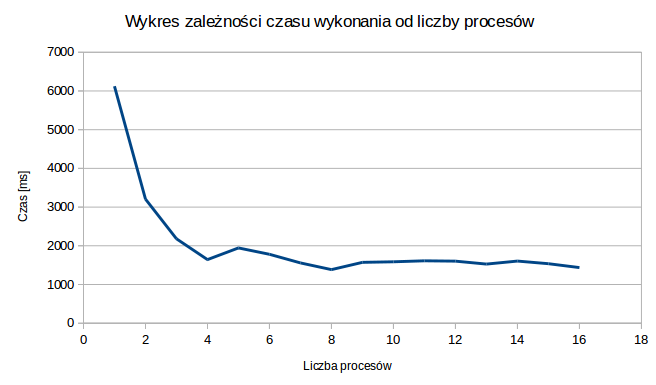
\includegraphics[width=0.75\textwidth]{dane/wykres1.png}
  \caption{Wykres zależności czasu wykonania od liczby procesów}
\end{figure}

Na wykresie można zaobserwować, że w czas wykonania malał gdy liczba procesów się zwiększała. Poprawę zanotowano dla pierwszych 4 procesów. Nieco wolniej malał aż do wykorzystania 8 procesów, po osiągnięciu których ustabilizował się. Wynika to z faktu, że największy zysk przyspieszenia uzyskujemy uruchamiając pierwsze dodatkowe rdzenie. Korzystając z większej ilości rdzeni, zysk nie jest już tak znaczący. Potwierdza to wykres przyspieszenia umieszczony poniżej.

\begin{figure}[H]
	\centering
  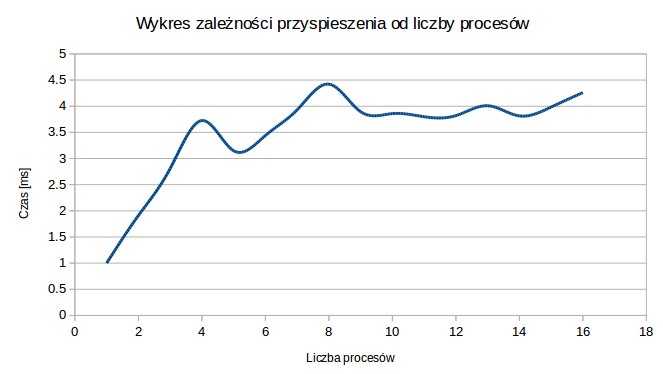
\includegraphics[width=0.75\textwidth]{dane/wykres2.png}
  \caption{Wykres zależności przyspieszenia od liczby procesów}
\end{figure}
 
Drugi wykres przedstawia zależność przyspieszenia od liczby procesów.Podobnie jak na pierwszym wykresie widać, że przyspieszenie poprawia się do 4 procesów, następnie spada, by później osiągnąć maksymalną wartość dla 8 procesów. \newline

Zadanie zostało w pełni zrealizowane, a otrzymane wyniki są zadowalające.
Zrównoleglając operacje przy użyciu interfejsu MPI udało się uzyskać niemalże 4,5 krotne przyspieszenie, co jest satysfakcjonującym wynikiem. Warto zauważyć także nieoczekiwany wzrost czasu wykonania dla wykonywania operacji na 5,6 oraz 7 procesach. Wynika to z faktu, że do dyspozycji mamy 4 rdzenie procesora.

\end{document}
